\section{Impact of non-DIS processes}
\label{app:nondis}

Among the event generators for muon- and neutrino-scattering considered in this work, only the dedicated neutrino generators (\genie, {\sc\small NuWro} and {\sc\small GiBUU}) account for non-DIS contributions: quasi-elastic, resonance, and diffractive scattering; here we use \genie to quantify these contributions.
%
Here we evaluate the size of these non-DIS effects for the observables relevant for this study, showing that they can be for all practical purposes neglected in FASER simulations. 

First, we consider total integrated cross-sections.
%
Table~\ref{tab:nondis} provides the percentage contribution to the total inclusive cross-section, evaluated with \genie, for NC muon DIS and CC neutrino DIS at three different values of $E_\ell$. 
  %
  The non-DIS processes are quasi-elastic scattering (QEL), resonance production (RES), and diffractive scattering (DFR).
%
For muon DIS we apply a $Q^2 > 4$~GeV$^2$ cut, while for neutrino DIS no such cut is necessary since \genie allows extrapolation down to $Q^2\to 0$. 
%
No cut on $W$, the invariant mass of the hadronic final state, is applied for the numbers quoted in this table.
%
For this calculation, the target is assumed to be a free proton. 

We find that for energies above a few hundred GeV, as relevant for FASER, the non-DIS channels contribute at the per-cent level or below, $1.5\%$ at most (for $\bar\nu_\mu$ at 400~GeV), and hence can be safely neglected, at least at the inclusive level.
%
For example, for $\nu_\mu$ CC scattering, their sum is 0.8\% of the total at 400~GeV, 0.3\% at 1~TeV and 0.1\% at 4~TeV, dominated at all energies by resonance production, while for $\bar\nu_\mu$ scattering this non-DIS contribution is about twice as large because its quasi-elastic channel is open on the proton.  
%
For muon DIS, for which the condition $Q^2> 4$~GeV$^2$ is imposed, non-DIS corrections are always below the 1\% level and are dominated by resonance production.
%
As in the neutrino case, also for NC scattering it is clear that non-DIS contributions are negligible for fiducial cross-sections. 
%
Note that in Table~\ref{tab:nondis} ``DIS'' is understood in the \genie sense, so also includes the SIS region at low $Q^2$ which is phenomenologically relevant for inclusive neutrino rates, cf.\ the discussion around Fig.~\ref{fig:faser-electronic}.

%%%%%%%%%%%%%%%%%%%%%%%
\begin{table}[!tbp]
  \centering
    \renewcommand{\arraystretch}{1.60}
  \begin{tabularx}{\textwidth}{X | ccc | ccc | ccc}
    \toprule
    & \multicolumn{3}{c|}{$\mu^-$ NC ($Q^2 > 4$~GeV$^2$)} & \multicolumn{3}{c|}{$\nu_\mu$ CC ($Q^2 > 0$)}  & \multicolumn{3}{c}{$\bar\nu_\mu$ CC ($Q^2 > 0$)} \\
    channel & 400~GeV & 1~TeV & 4~TeV & 400~GeV & 1~TeV & 4~TeV & 400~GeV & 1~TeV & 4~TeV \\
    \midrule
    DIS  (\%)        & 99.20 & 99.42 & 99.62 & 99.25 & 99.68 & 99.91 & 98.48 & 99.37 & 99.83 \\
    \midrule
    RES   (\%)       &  0.75 &  0.54 &  0.36 &  0.58 &  0.24 &  0.07 &  0.78 &  0.32 &  0.09 \\
    QEL   (\%)       &  0.05 &  0.03 &  0.02 &  0.01 & 0.005 & 0.001 &  0.56 &  0.23 &  0.06 \\
    DFR   (\%)       & ---   & ---   & ---   &  0.16 &  0.08 &  0.03 &  0.18 &  0.09 &  0.03 \\
    \midrule
    non-DIS total (\%)    &  0.80 &  0.58 &  0.38 &  0.75 &  0.32 &  0.09 &  1.52 &  0.63 &  0.17 \\
    \bottomrule
  \end{tabularx}
  \vspace{0.3cm}
  \caption{Percentage contribution to the total inclusive cross-section, evaluated with \genie, for NC muon DIS and CC neutrino DIS at three different values of $E_\ell$.
  %
  The non-DIS processes are QEL, RES and DFR.
%
For muon DIS we apply a $Q^2 > 4$~GeV$^2$ cut, while for neutrino DIS no such cut is necessary since \genie allows extrapolation down to $Q^2\to 0$. 
%
No cut on $W$, the invariant mass of the hadronic final state, is applied for the numbers quoted in this table.
%
Here DIS is understood in the \genie sense, and hence includes also the SIS region at low $Q^2$ (see text).
}
  \label{tab:nondis}
\end{table}
%%%%%%%%%%%%%%%%%%%%%%%

Then Fig.~\ref{fig:nondis} shows the corresponding differential distributions in $Q^2$, $W$, and $x_{\rm Bj}$ evaluated with \genie (GRV98LO tune) for muon NC and muon-neutrino CC scattering  for $E_\ell=100$ GeV and $E_\ell=1$ TeV including non-DIS contributions, now per nucleon on a tungsten target rather than on the free proton of Table~\ref{tab:nondis}. 
%
In this case, and as opposed to Table~\ref{tab:nondis}, only events that fall inside the fiducial region of the benchmark, namely  $Q^2 > 4$~GeV$^2$ and $W > 3$~GeV, are retained. 
%
For each distribution, the bottom panels indicate the relative contribution of non-DIS processes to the predicted bin yields.
%
In the case of muon DIS, this contribution is exactly zero within the statistics of the generated sample, since all non-DIS contributions fall outside the considered fiducial region and \genie does not simulate diffractive scattering for charged leptons. 
%
For neutrino DIS, the only non-DIS contribution which survives is diffractive scattering, which is nevertheless below the per-mille level for all distributions at both values of $E_\nu$.
%
Hence from Fig.~\ref{fig:nondis} we conclude that also for differential distributions in the fiducial region Eq.~(\ref{eq:fiducial}) all non-DIS processes can be safely neglected when producing predictions for FASER observables.  

%%%%%%%%%%%%%%%%%%%%%%%%%%%%%%%%%%%%%
\begin{figure}[!tbp]
  \centering
  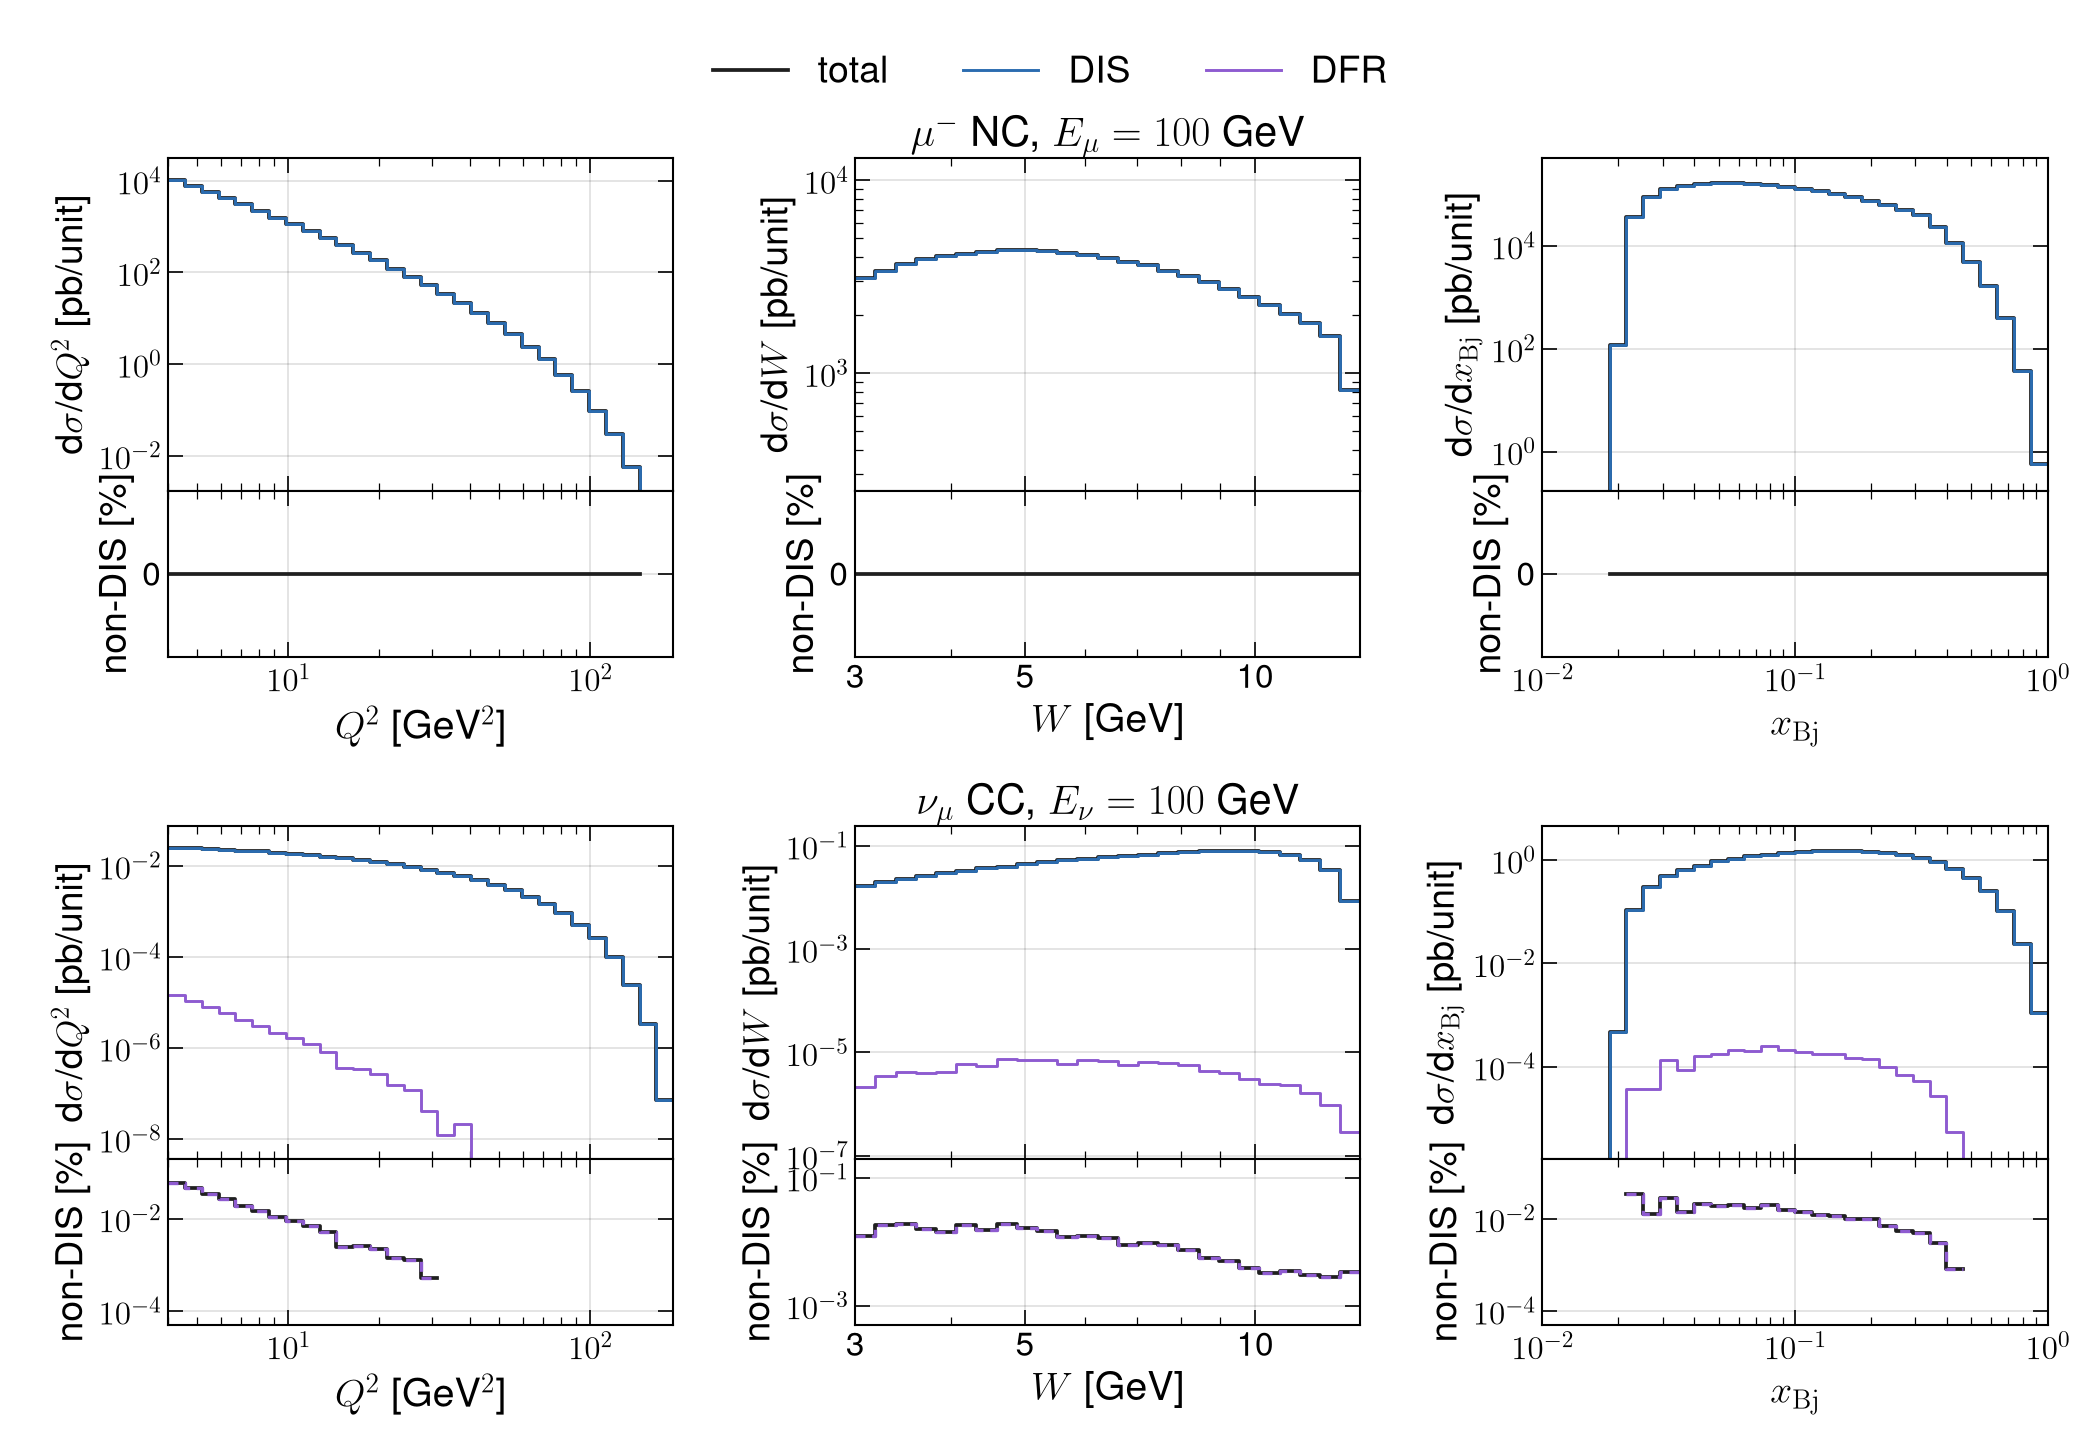
\includegraphics[width=0.94\textwidth]{figures/pp_genie_nondis_100GeV.png}
  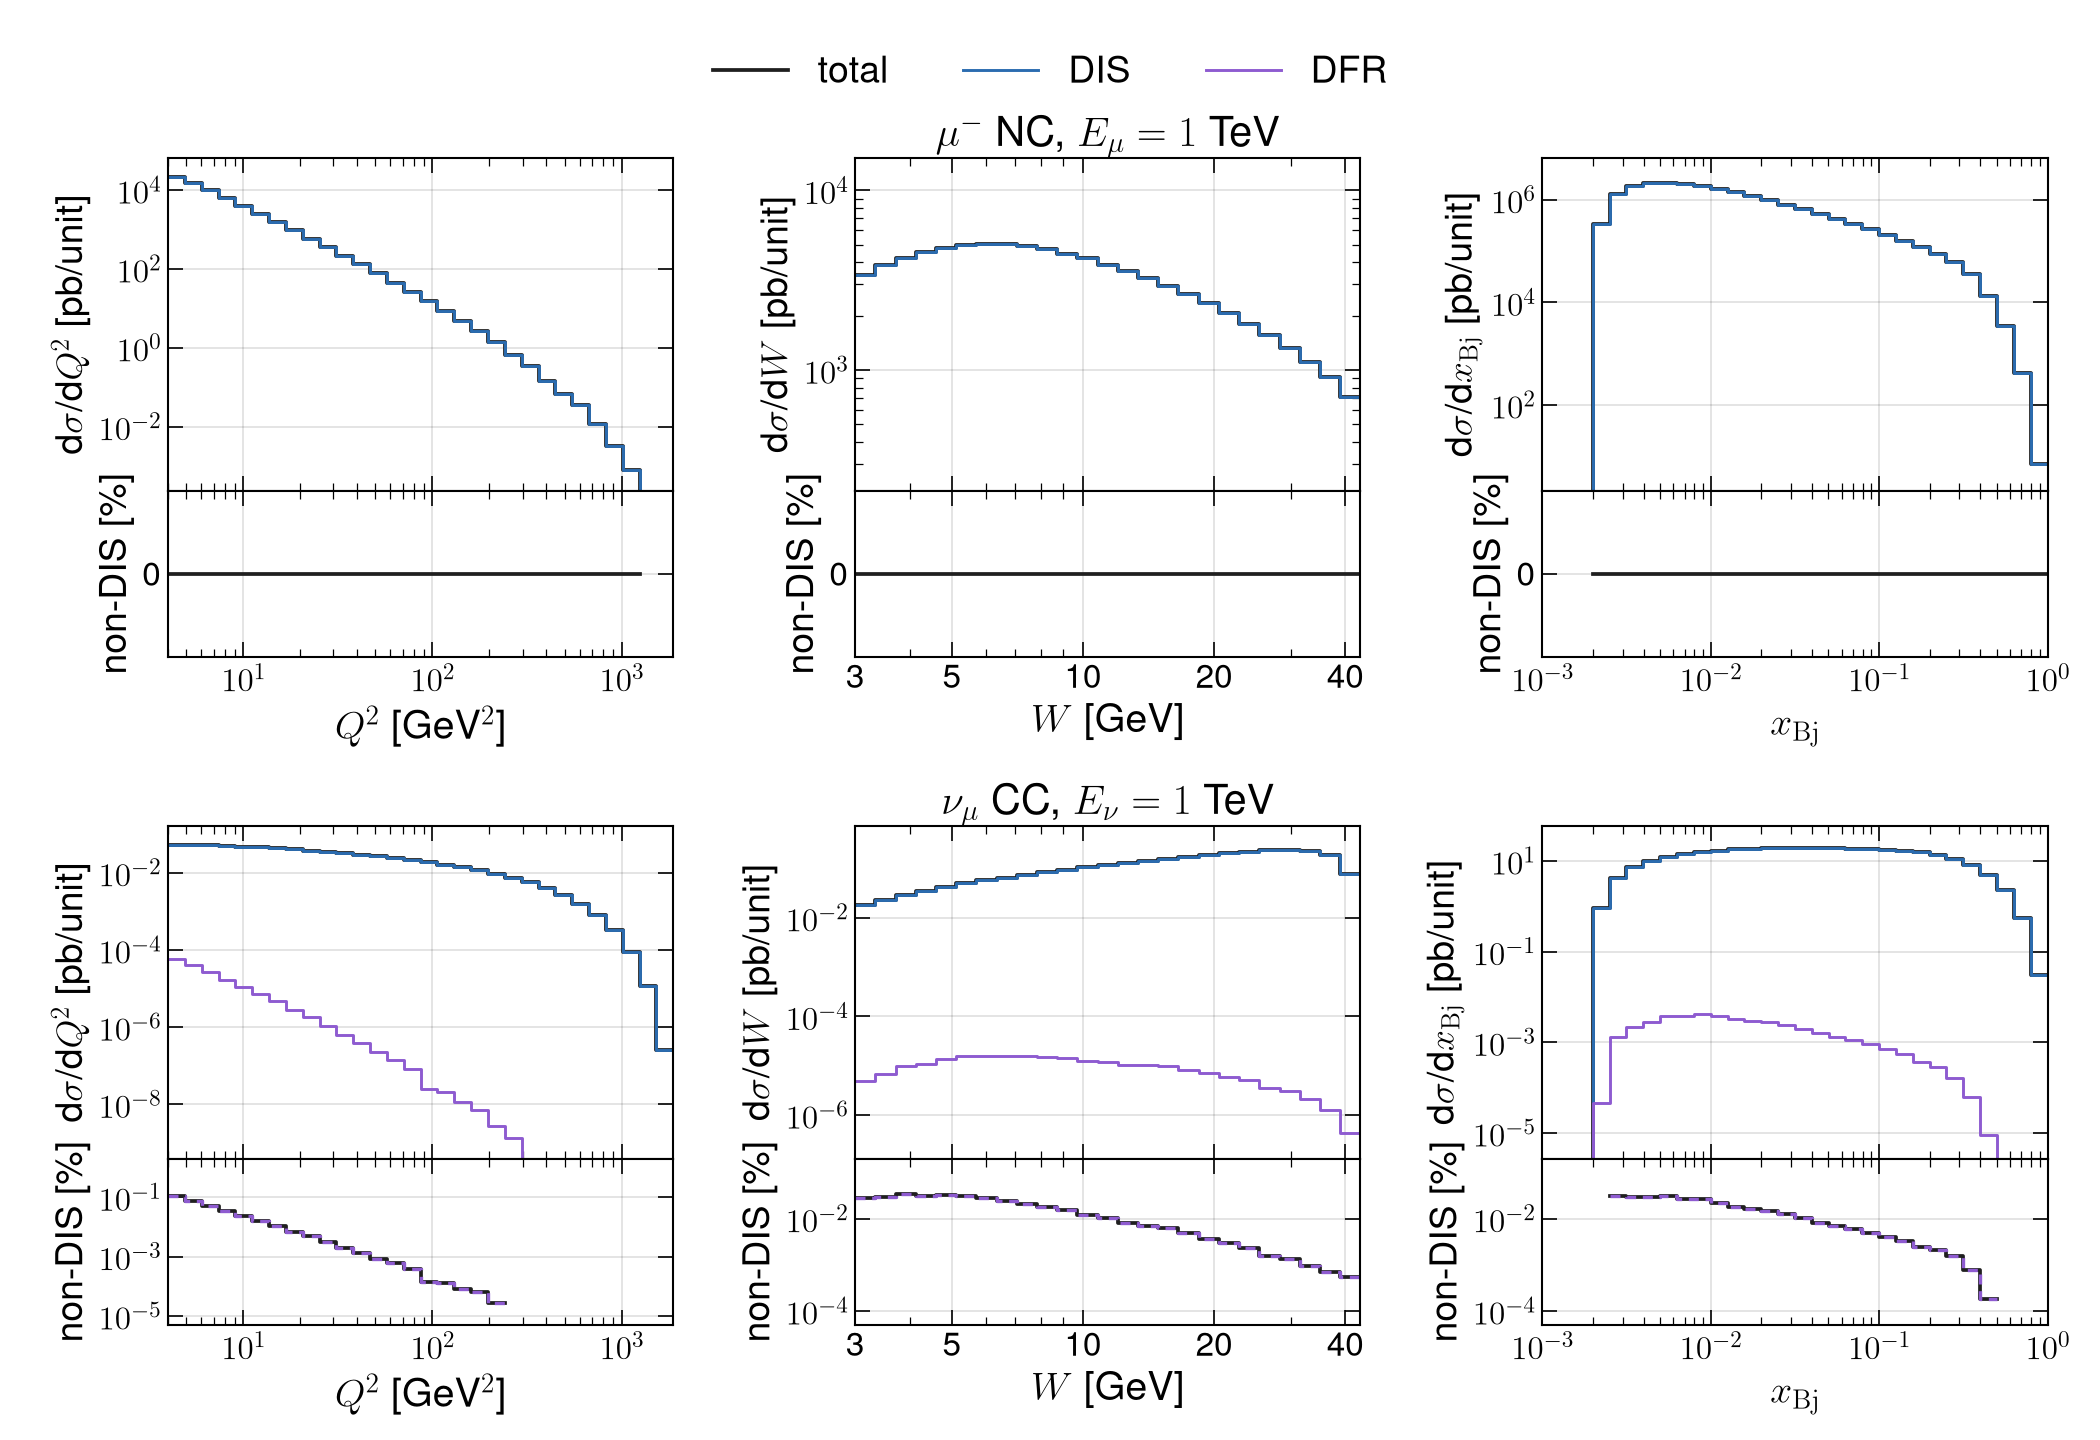
\includegraphics[width=0.94\textwidth]{figures/pp_genie_nondis.png}
  \caption{Differential distributions in $Q^2$, $W$, and $x_{\rm Bj}$ evaluated with \genie (GRV98LO) per nucleon on a tungsten target for muon NC and muon-neutrino CC scattering  for $E_\ell=100$ GeV (top panels) and $E_\ell=1$ TeV (bottom panels), including also non-DIS contributions. 
%
Only events that fall inside the fiducial region of  $Q^2 > 4$~GeV$^2$ and $W > 3$~GeV are retained. 
%
For each distribution, the bottom panels indicate the relative contribution of non-DIS processes to the predicted bin yields: in the case of muon DIS, this contribution is exactly zero within the statistics of the generated sample.
}
  \label{fig:nondis}
\end{figure}
%%%%%%%%%%%%%%%%%%%%%%%%%

We also note that  \genie labels as DIS the whole inelastic continuum, including the SIS region at low $Q^2$ where perturbative QCD is not applicable, as well as the non-resonant background below the $W$ cut of the fiducial selection, Eq.~(\ref{eq:fiducial}). 
%
The contribution of this SIS region for a tungsten target is not negligible: between 3 and 6\% of the neutrino inelastic scattering channel (both DIS in the benchmark sense and SIS) sits below $Q^2 = 4$~GeV$^2$ at $E_\nu=400$~GeV and 1~TeV, while more than 99.5\% of it lies above $W = 2$~GeV; at $E_\nu=100$~GeV these fractions are 17\% and 98\% respectively.  
%
Hence, while the contributions from outside the DIS region in the sense of Eq.~(\ref{eq:fiducial}), namely the SIS region together with the non-DIS processes of Table~\ref{tab:nondis}, are not negligible for fully inclusive FASER neutrino cross-sections, they become negligible once cuts in $Q^2$ and $W$ ensuring the validity of the perturbative QCD calculations are applied.

However, the cuts of Eq.~(\ref{eq:fiducial}) can often not be applied, for instance in measurements in which only the outgoing muon is reconstructed, such as the electronic-detector analysis of Fig.~\ref{fig:faser-electronic}.
%
It is therefore useful to quantify how CC interactions are distributed among the different kinematic regions, as done in~\cite{Feng:2022inv} with \pythia alone.
%
Table~\ref{tab:kin-regions} reports, for $\nu_\mu$ and $\bar\nu_\mu$ CC scattering on tungsten evaluated with the default \genie tune and including all channels, the fraction of events in the DIS region ($Q^2>4$~GeV$^2$ and $W>2$~GeV), split into the fiducial region of the benchmark ($W>3$~GeV) and the strip $2<W<3$~GeV; in the SIS region ($Q^2<4$~GeV$^2$ and $W>2$~GeV); and in the resonance region ($W<2$~GeV), which contains the QEL and RES channels together with the non-resonant inelastic background.
%
These fractions are given at $E_\nu=100$~GeV and 1~TeV, as well as weighted with the FASER$\nu$ Run~3 flux of Sect.~\ref{sec:faser-app}, that is, as fractions of the expected number of CC interactions.

%%%%%%%%%%%%%%%%%%%%%%%
\begin{table}[!tbp]
  \centering
  \small
  \renewcommand{\arraystretch}{1.50}
  \begin{tabularx}{\textwidth}{X | ccc | ccc}
    \toprule
    & \multicolumn{3}{c|}{$\nu_\mu$ CC} & \multicolumn{3}{c}{$\bar\nu_\mu$ CC} \\
    region & 100~GeV & 1~TeV & FASER$\nu$ flux & 100~GeV & 1~TeV & FASER$\nu$ flux \\
    \midrule
    DIS: $Q^2>4$ GeV$^2$ \& $W>3$~GeV (\%)& 79.5 & 96.5 & 90.8 & 62.9 & 93.4 & 82.3 \\
    DIS: $Q^2>4$ GeV$^2$ \& $2<W<3$~GeV (\%)            &  1.3 & 0.14 & 0.56 &  2.3 & 0.28 & 0.97 \\
    SIS: $Q^2<4$ GeV$^2$ \& $W > 2$ GeV (\%)                         & 15.5 &  3.0 &  7.2 & 27.5 &  5.7 & 13.5 \\
    Resonance region: $W<2$~GeV (\%)       &  3.6 & 0.31 &  1.5 &  7.3 & 0.62 &  3.2 \\
    \bottomrule
  \end{tabularx}
  \vspace{0.3cm}
  \caption{Fraction of $\nu_\mu$ and $\bar\nu_\mu$ CC interactions on tungsten in each kinematic region, evaluated with the default \genie tune including all channels (that is, also with the RES, QEL and DFR processes of Table~\ref{tab:nondis}).
  %
  We show results at two fixed energies, $E_\nu=100$~GeV and 1~TeV, and weighted with the FASER$\nu$ Run~3 flux used in Sect.~\ref{sec:faser-app}.
  %
  In this table, DIS denotes $Q^2>4$~GeV$^2$ and $W>2$~GeV, split into the fiducial region of the benchmark, Eq.~(\ref{eq:fiducial}), and the strip $2<W<3$~GeV; SIS denotes the region defined by $Q^2<4$~GeV$^2$ and $W>2$~GeV; and the resonance region corresponds to $W<2$~GeV, which contains the QEL and RES channels together with the non-resonant inelastic background.
  %
  The kinematic variables are reconstructed from the outgoing muon.
}
  \label{tab:kin-regions}
\end{table}
%%%%%%%%%%%%%%%%%%%%%%%

Weighted with the predicted flux, about $90\%$ ($80\%$) of the $\nu_\mu$ ($\bar\nu_\mu$) CC interactions fall inside the fiducial region of the benchmark and are hence described by the NLO-matched generators studied in this work, while the SIS region accounts for $7\%$ ($13\%$) and the resonance region for $1.5\%$ ($3\%$) of the events.
%
The fraction of events outside the fiducial region grows rapidly as the energy decreases, from $3\%$ ($7\%$) at $E_\nu=1$~TeV to $20\%$ ($37\%$) at 100~GeV and to about one half (three quarters) at 30~GeV, consistently with the size of the SIS ($Q^2<4$~GeV$^2$) contribution added to the NLO predictions in Fig.~\ref{fig:faser-electronic}.
%
The strip $2<W<3$~GeV between the conventional DIS boundary and the benchmark cut is at most $5\%$ at any energy and below $1\%$ after flux weighting.
